\chapter{Équilibres acido-basiques et méthode de la réaction prépondérante}\label{ch:b1:predominant-reaction}

Le vinaigre dissout le tartre d'une bouilloire~; le jus de citron aussi,
un peu plus vite. Le sang maintient son pH entre des limites étroites,
quoi que l'on mange~; une boisson gazeuse est acide à cause du dioxyde
de carbone qui y est dissous. Ce sont autant d'équilibres acido-basiques
dans l'eau, et le chimiste qui doit traiter une solution contenant
plusieurs acides et plusieurs bases --- un mélange, un tampon, un
\omterm{def:b1:predominant-reaction:polyprotic}{polyacide} --- a besoin d'une méthode sûre pour en trouver le pH et les
concentrations des espèces. Ce chapitre construit cette méthode~: une
échelle de forces, des \omterm{def:b1:predominant-reaction:predominance}{diagrammes de prédominance}, et la \emph{méthode
de la \omterm{def:b1:predominant-reaction:predominant-reaction}{réaction prépondérante}}, qui ramène tout mélange à la seule
réaction qui compte.

\begin{recall}
Le livre 1 (année 12) a défini les acides et les \omterm{def:b1:predominant-reaction:bronsted}{bases de Brønsted}, la
\omterm{def:b1:predominant-reaction:acidity-constant}{constante d'acidité} $K_a$ et le $\mathrm{p}K_a$, le \omterm{def:b1:predominant-reaction:autoprotolysis}{produit ionique de
l'eau} et le pH des acides et des bases forts, et tracé des \omterm{def:b1:predominant-reaction:predominance}{diagrammes de
prédominance}. Le \omterm{def:b1:extent-q-and-k:quotient}{quotient de réaction}, la constante d'équilibre et les
\omterm{def:b1:extent-q-and-k:activity}{activités} des solutés ($c/c^\circ$) et du solvant (1) ont été définis au
\cref{ch:b1:extent-q-and-k}~; dans ce chapitre, on n'écrit pas
$c^\circ = \qty{1}{mol/L}$ dans les quotients.
\end{recall}

\begin{omfigure}
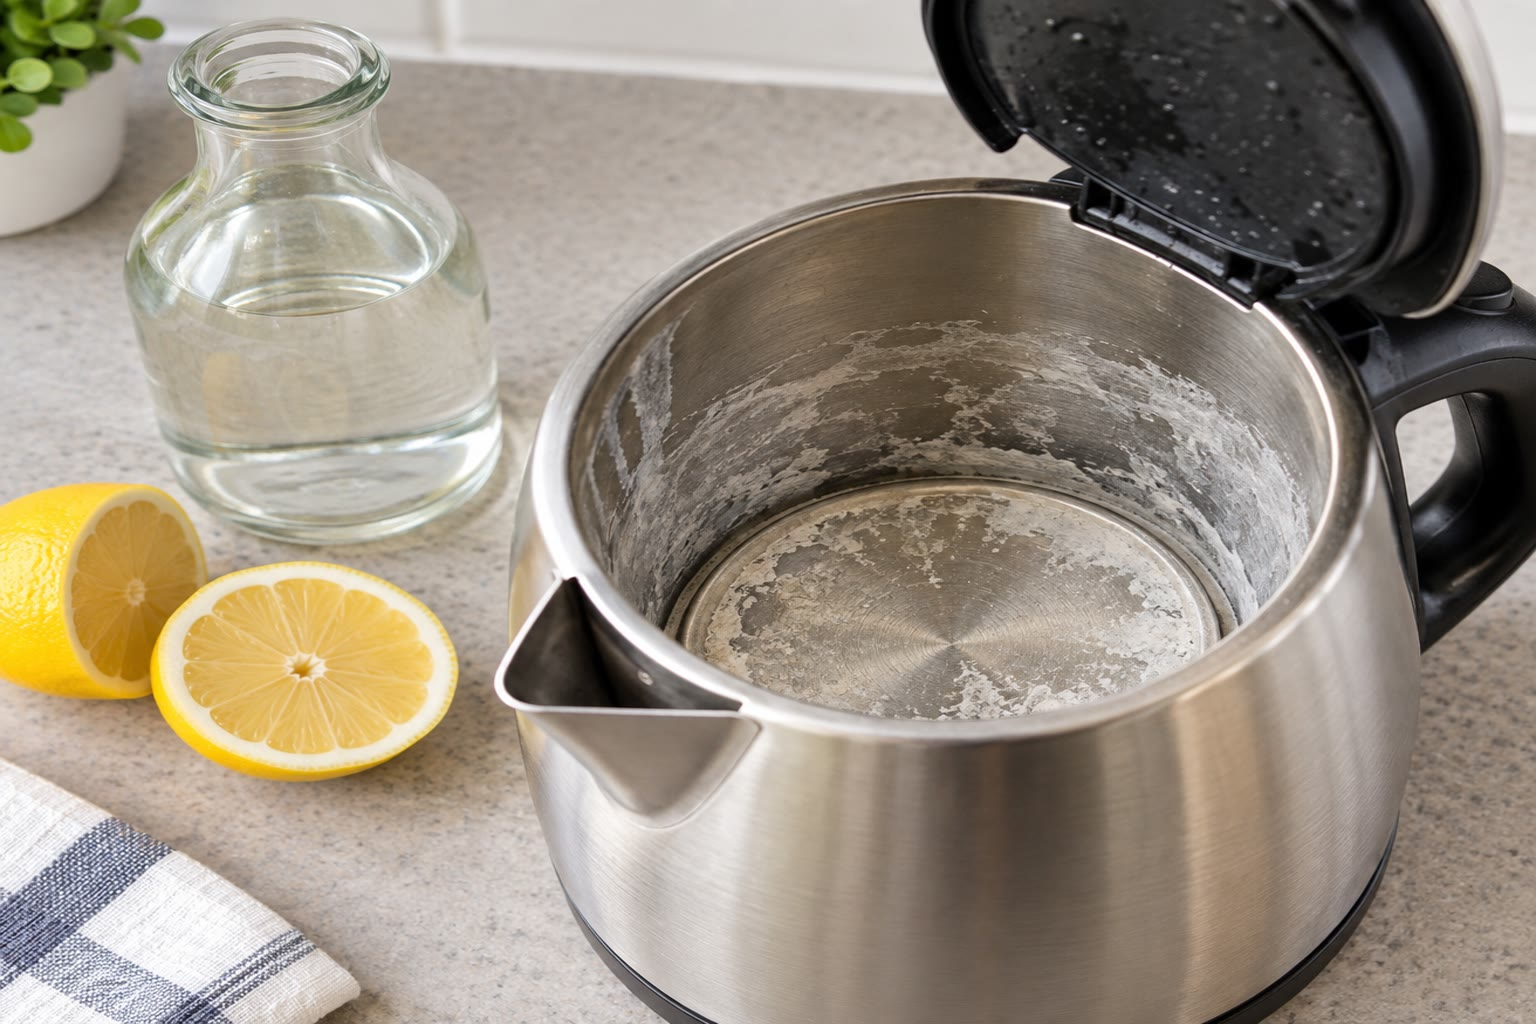
\includegraphics[width=0.5\linewidth]{images/book2/ai/b1-10-descaling.jpg}

{\small Du tartre, du carbonate de calcium, dans une bouilloire. Les
\omterm{def:b1:predominant-reaction:strong-acid}{acides faibles} du vinaigre et du jus de citron réagissent avec l'ion
carbonate et le dissolvent.}
\end{omfigure}

\section{Couples de Brønsted et pH}

\begin{definition}[Acide et base de Brønsted, couple]\label{def:b1:predominant-reaction:bronsted}
Un \emph{acide de Brønsted}\index{acide de Bronsted@acide de Brønsted} est une espèce capable de céder un
proton \ce{H+}~; une \emph{base de Brønsted}\index{base de Bronsted@base de Brønsted} est une espèce
capable d'en capter un. Un acide HA et la base A qu'il devient en perdant
un proton forment un \emph{couple acide/base}\index{couple acide/base} HA/A,
reliés par la demi-équation formelle $\mathrm{HA} \rightleftharpoons
\mathrm{A} + \ce{H+}$. Dans l'eau, le proton n'est jamais libre~: il est
porté par une molécule d'eau, sous la forme \ce{H3O+}.
\end{definition}

\begin{definition}[Ampholyte]\label{def:b1:predominant-reaction:ampholyte}
Un \emph{ampholyte}\index{ampholyte} (une espèce amphotère) est la base
d'un couple et l'acide d'un autre~: l'eau (\ce{H3O+}/\ce{H2O} et
\ce{H2O}/\ce{OH-}), l'ion hydrogénocarbonate (\ce{CO2,H2O}/\ce{HCO3-}
et \ce{HCO3-}/\ce{CO3^{2-}}), l'ion dihydrogénophosphate.
\end{definition}

\begin{definition}[Autoprotolyse, produit ionique, pH]\label{def:b1:predominant-reaction:autoprotolysis}
L'eau subit l'\emph{autoprotolyse}\index{autoprotolyse},
\ce{2H2O <=> H3O+ + OH-}, de constante $K_e = [\ce{H3O+}][\ce{OH-}]$, le
\emph{produit ionique de l'eau}\index{produit ionique de l'eau}~; à
\qty{25}{\celsius}, $K_e = 10^{-14.00}$, donc $\mathrm{p}K_e = 14.00$. Le
pH d'une solution vaut $\mathrm{pH} = -\log a(\ce{H3O+}) \approx -\log[\ce{H3O+}]$.
Une solution est neutre lorsque $[\ce{H3O+}] = [\ce{OH-}]$, c'est-à-dire
à $\mathrm{pH} = \mathrm{p}K_e/2 = 7.00$ à \qty{25}{\celsius}.
% ledger: dfg:H2O_l, dfg:OH-_ao (pKe computed in figdata/bachelor-1/aqueous-constants.py)
\end{definition}

\section{Force~: \texorpdfstring{$K_a$}{Ka}, \texorpdfstring{p$K_a$}{pKa} et effet nivelant}

\begin{definition}[Constante d'acidité]\label{def:b1:predominant-reaction:acidity-constant}
La \emph{constante d'acidité}\index{constante d'acidite@constante d'acidité} d'un couple HA/A est
la constante de la réaction de l'acide avec l'eau,
\[
  \mathrm{HA} + \ce{H2O} \rightleftharpoons \mathrm{A} + \ce{H3O+}, \qquad
  K_a = \frac{[\mathrm{A}][\ce{H3O+}]}{[\mathrm{HA}]}, \qquad
  \mathrm{p}K_a = -\log K_a .
\]
Plus $K_a$ est grande (plus le $\mathrm{p}K_a$ est petit), plus l'acide
est fort et plus sa base conjuguée est faible.
\end{definition}

\begin{definition}[Acides et bases forts et faibles]\label{def:b1:predominant-reaction:strong-acid}
Un acide est \emph{fort}\index{acide fort} dans l'eau si sa réaction avec
l'eau est totale~: il ne reste aucune molécule HA (acides chlorhydrique,
nitrique, perchlorique, première acidité de l'acide sulfurique)~; sinon,
il est \emph{faible}\index{acide faible}. Une base est \emph{forte}\index{base forte}
si sa réaction avec l'eau est totale et donne \ce{OH-} (hydroxydes, ion
oxyde, alcoolates), et \emph{faible}\index{base faible} sinon.
\end{definition}

\begin{definition}[Effet nivelant]\label{def:b1:predominant-reaction:levelling}
Dans l'eau, tout acide plus fort que \ce{H3O+} réagit totalement pour
donner \ce{H3O+}, et toute base plus forte que \ce{OH-} totalement pour
donner \ce{OH-}~: on ne peut plus distinguer leurs forces. C'est
l'\emph{effet nivelant}\index{effet nivelant} du solvant. Les acides et
les \omterm{def:b1:predominant-reaction:strong-acid}{bases faibles} dans l'eau ont $0 < \mathrm{p}K_a < 14$, les couples
de l'eau elle-même ($\mathrm{p}K_a(\ce{H3O+}/\ce{H2O}) = 0$ et
$\mathrm{p}K_a(\ce{H2O}/\ce{OH-}) = 14$) bornant l'échelle.
\end{definition}

\begin{center}
\small
\begin{tabular}{lll@{\hspace{2.5em}}lll}
\hline
couple & p$K_a$ & & couple & p$K_a$ & \\
\hline
\ce{HSO4-}/\ce{SO4^{2-}} & 1.99 & & \ce{CO2,H2O}/\ce{HCO3-} & 6.37 & \\
\ce{H3PO4}/\ce{H2PO4-} & 2.15 & & \ce{H2PO4-}/\ce{HPO4^{2-}} & 7.21 & \\
\ce{HF}/\ce{F-} & 3.16 & & \ce{HClO}/\ce{ClO-} & 7.55 & \\
\ce{HCOOH}/\ce{HCOO-} & 3.74 & & \ce{NH4+}/\ce{NH3} & 9.25 & \\
\ce{CH3COOH}/\ce{CH3COO-} & 4.76 & & \ce{C6H5OH}/\ce{C6H5O-} & 9.99 & \\
\ce{C6H5NH3+}/\ce{C6H5NH2} & 4.60 & & \ce{HCO3-}/\ce{CO3^{2-}} & 10.33 & \\
\ce{C6H5COOH}/\ce{C6H5COO-} & 4.21 & & \ce{CH3NH3+}/\ce{CH3NH2} & 10.66 & \\
\hline
\end{tabular}
\end{center}
% ledger: pka:methanoic, pka:ethanoic, pka:anilinium, pka:benzoic,
% pka:phenol, pka:methylammonium (IUPAC dataset); dfg:HSO4-_ao,
% dfg:SO42-_ao, dfg:H3PO4_ao, dfg:H2PO4-_ao, dfg:HPO42-_ao, dfg:HF_ao,
% dfg:F-_ao, dfg:CO2_ao, dfg:HCO3-_ao, dfg:CO32-_ao, dfg:HClO_ao,
% dfg:ClO-_ao, dfg:NH4+_ao, dfg:NH3_ao (pKa computed from NBS-82)

\section{Diagrammes de prédominance et de distribution}

\begin{definition}[Diagrammes de prédominance et de distribution]\label{def:b1:predominant-reaction:predominance}
Pour un couple HA/A, $\mathrm{pH} = \mathrm{p}K_a + \log([\mathrm{A}]/[\mathrm{HA}])$~:
l'acide prédomine ($[\mathrm{HA}] > [\mathrm{A}]$) pour
$\mathrm{pH} < \mathrm{p}K_a$, la base pour $\mathrm{pH} > \mathrm{p}K_a$.
Le \emph{diagramme de prédominance}\index{diagramme de predominance@diagramme de prédominance} est l'axe des pH
partagé à chaque $\mathrm{p}K_a$ en domaines où prédomine chacune des
formes. Le \emph{diagramme de distribution}\index{diagramme de distribution}
donne la fraction de chaque forme, $[\text{forme}]/C$, en fonction du pH.
\end{definition}

\begin{proposition}[La relation de Henderson et les fractions]\label{prop:b1:predominant-reaction:henderson}
Pour un couple HA/A de concentration totale $C = [\mathrm{HA}] + [\mathrm{A}]$,
\[
  \mathrm{pH} = \mathrm{p}K_a + \log\frac{[\mathrm{A}]}{[\mathrm{HA}]}, \qquad
  \frac{[\mathrm{HA}]}{C} = \frac{1}{1 + 10^{\mathrm{pH} - \mathrm{p}K_a}}, \qquad
  \frac{[\mathrm{A}]}{C} = \frac{1}{1 + 10^{\mathrm{p}K_a - \mathrm{pH}}} .
\]
À une unité de pH du $\mathrm{p}K_a$, la forme minoritaire représente
moins de 10\,\% du total~; à deux unités, moins de 1\,\%.
\end{proposition}

\begin{proof}
On prend le logarithme de $K_a = [\mathrm{A}][\ce{H3O+}]/[\mathrm{HA}]$.
Alors
$[\mathrm{A}]/[\mathrm{HA}] = 10^{\mathrm{pH}-\mathrm{p}K_a}$, et la
division de
$[\mathrm{HA}]$ par $[\mathrm{HA}] + [\mathrm{A}]$ donne les fractions. À
$\mathrm{pH} = \mathrm{p}K_a + 1$, $[\mathrm{HA}]/C = 1/11 < 10\,\%$~; à
$+2$, $1/101$.
\end{proof}

\begin{omfigure}
\begin{tikzpicture}
\begin{axis}[name=e,
  width=0.48\linewidth, height=5.2cm, xmin=0, xmax=14, ymin=0, ymax=1.05,
  axis x line=bottom, axis y line=left, xlabel={pH}, ylabel={fraction},
  xtick={0,2,4,6,8,10,12,14},
  tick label style={font=\small}, label style={font=\small}]
\addplot[omDef, thick] table[x=pH, y=HA] {figdata/out/bachelor-1-distribution-diagrams-ethanoic.dat};
\addplot[omThm, thick] table[x=pH, y=A] {figdata/out/bachelor-1-distribution-diagrams-ethanoic.dat};
\draw[dotted] (axis cs:4.76,0) -- (axis cs:4.76,0.5);
\node[omDef, font=\footnotesize, anchor=west] at (axis cs:0.3,0.3) {\ce{CH3COOH}};
\node[omThm, font=\footnotesize, anchor=east] at (axis cs:13.7,0.3) {\ce{CH3COO-}};
\node[font=\small, anchor=north west] at (axis cs:4.8,0.48) {4.76};
\end{axis}
\begin{axis}[at={(e.east)}, anchor=west, xshift=1.1cm,
  width=0.48\linewidth, height=5.2cm, xmin=0, xmax=14, ymin=0, ymax=1.05,
  axis x line=bottom, axis y line=left, xlabel={pH}, ylabel={fraction},
  xtick={0,2,4,6,8,10,12,14},
  legend style={font=\scriptsize, draw=none, at={(0.5,1.04)}, anchor=south, legend columns=4},
  tick label style={font=\small}, label style={font=\small}]
\addplot[omDef, thick] table[x=pH, y=H3A] {figdata/out/bachelor-1-distribution-diagrams-phosphoric.dat};
\addplot[omMeth, thick] table[x=pH, y=H2A] {figdata/out/bachelor-1-distribution-diagrams-phosphoric.dat};
\addplot[omProp, thick] table[x=pH, y=HA] {figdata/out/bachelor-1-distribution-diagrams-phosphoric.dat};
\addplot[omThm, thick] table[x=pH, y=A] {figdata/out/bachelor-1-distribution-diagrams-phosphoric.dat};
\legend{\ce{H3PO4}, \ce{H2PO4-}, \ce{HPO4^{2-}}, \ce{PO4^{3-}}}

\end{axis}
\end{tikzpicture}

\begin{tikzpicture}[font=\small, >={Stealth}]
  \draw[->, thick] (0,0) -- (14.2*0.85,0) node[right] {pH};
  \foreach \x/\l in {2.15/2.15, 7.21/7.21, 12.34/12.34}
    \draw (\x*0.85,0.15) -- (\x*0.85,-0.15) node[below] {\l};
  \node[above] at (1.07*0.85,0.1) {\ce{H3PO4}};
  \node[above] at (4.68*0.85,0.1) {\ce{H2PO4-}};
  \node[above] at (9.78*0.85,0.1) {\ce{HPO4^{2-}}};
  \node[above] at (13.3*0.85,0.1) {\ce{PO4^{3-}}};
\end{tikzpicture}

{\small \omterm{def:b1:predominant-reaction:predominance}{Diagrammes de distribution} de l'acide éthanoïque (à gauche) et
de l'acide phosphorique (à droite), et \omterm{def:b1:predominant-reaction:predominance}{diagramme de prédominance} de
l'acide phosphorique. Chaque croisement de deux courbes voisines se
trouve à un $\mathrm{p}K_a$~; les \omterm{def:b1:predominant-reaction:ampholyte}{ampholytes} \ce{H2PO4-} et
\ce{HPO4^{2-}} sont presque la seule forme présente au milieu de leurs
domaines.}
\end{omfigure}

% fr layout: keeps the heading off the foot of the page
\clearpage
\section{La méthode de la réaction prépondérante}

\begin{proposition}[Constante d'une réaction acido-basique]\label{prop:b1:predominant-reaction:k-of-reaction}
La réaction de l'acide $\mathrm{HA}_1$ d'un couple sur la base
$\mathrm{A}_2$ d'un autre,
$\mathrm{HA}_1 + \mathrm{A}_2 \rightleftharpoons \mathrm{A}_1 + \mathrm{HA}_2$,
a pour constante
\[
  K = \frac{K_{a1}}{K_{a2}} = 10^{\,\mathrm{p}K_{a2} - \mathrm{p}K_{a1}} .
\]
Elle est favorable ($K > 1$) lorsque l'acide est plus fort que l'acide
formé ($\mathrm{p}K_{a1} < \mathrm{p}K_{a2}$), et \omterm{def:b1:extent-q-and-k:quantitative}{quantitative} (au sens
de la \cref{met:b1:extent-q-and-k:quantitative}) lorsque l'écart des
$\mathrm{p}K_a$ dépasse 4 environ.
\end{proposition}

\begin{proof}
La réaction est la somme de $\mathrm{HA}_1 + \ce{H2O} \rightleftharpoons
\mathrm{A}_1 + \ce{H3O+}$ ($K_{a1}$) et de l'inverse de $\mathrm{HA}_2 +
\ce{H2O} \rightleftharpoons \mathrm{A}_2 + \ce{H3O+}$ ($1/K_{a2}$)~;
la \cref{prop:b1:extent-q-and-k:combine-k} donne $K = K_{a1}/K_{a2}$.
\end{proof}

\begin{definition}[Réaction prépondérante, solution équivalente]\label{def:b1:predominant-reaction:predominant-reaction}
Dans une solution qui contient plusieurs acides et plusieurs bases, la
\emph{réaction prépondérante}\index{reaction preponderante@réaction prépondérante} est la réaction de plus grande
constante entre l'acide le plus fort et la base la plus forte présents.
Lorsqu'elle est \omterm{def:b1:extent-q-and-k:quantitative}{quantitative}, on la traite comme totale, et l'on
remplace la solution par la \emph{solution équivalente}\index{solution equivalente@solution équivalente}~: la
solution obtenue une fois cette réaction achevée, qui a le même pH que
la solution réelle.
\end{definition}

\begin{method}[La méthode de la réaction prépondérante]\label{met:b1:predominant-reaction:method}
Pour déterminer le pH et la composition d'une solution~:
\begin{enumerate}
  \item recenser les espèces introduites (et l'eau) et placer leurs
        couples sur une échelle de $\mathrm{p}K_a$, les acides d'un côté,
        les bases de l'autre~;
  \item repérer l'acide le plus fort et la base la plus forte présents~;
  \item si la constante de leur réaction est grande ($K > 10^4$, ou
        $\Delta\mathrm{p}K_a > 4$), traiter la réaction comme totale et
        écrire la \omterm{def:b1:predominant-reaction:predominant-reaction}{solution équivalente}~; revenir à l'étape 2~;
  \item lorsque la \omterm{def:b1:predominant-reaction:predominant-reaction}{réaction prépondérante} a une faible constante, c'est
        elle qui fixe le pH~: dresser son tableau d'\omterm{def:b1:extent-q-and-k:extent}{avancement} et résoudre
        $Q = K$, en général avec l'hypothèse d'un faible \omterm{def:b1:extent-q-and-k:extent}{avancement}~;
  \item vérifier les hypothèses~: les espèces minoritaires le sont
        bien, et les autres réactions (y compris l'\omterm{def:b1:predominant-reaction:autoprotolysis}{autoprotolyse} de
        l'eau) sont négligeables.
\end{enumerate}
\end{method}

\begin{omfigure}
\begin{tikzpicture}[font=\small, >={Stealth}]
  \draw[->, thick] (0,-0.3) -- (0,7.6) node[above] {p$K_a$};
  \foreach \y/\a/\b in {0/\ce{H3O+}/\ce{H2O}, 1.58/\ce{HF}/\ce{F-}, 2.38/\ce{CH3COOH}/\ce{CH3COO-},
      3.62/\ce{H2PO4-}/\ce{HPO4^{2-}}, 4.62/\ce{NH4+}/\ce{NH3}, 7/\ce{H2O}/\ce{OH-}} {
    \draw (-0.12,\y) -- (0.12,\y);
    \node[anchor=east] at (-0.2,\y) {\a};
    \node[anchor=west] at (0.2,\y) {\b};
  }
  \foreach \y/\l in {0/0, 1.58/3.16, 2.38/4.76, 3.62/7.21, 4.62/9.25, 7/14} \node[black!60, anchor=west] at (3.0,\y) {\l};
  \draw[->, omThm, thick] (-1.6,2.55) -- (1.2,4.45);
  \node[omThm, anchor=west, align=left] at (4.2,3.5) {un acide réagit avec toute\\base placée au-dessus~: $K > 1$};
  \node[anchor=south] at (-1.4,7.35) {acides};
  \node[anchor=south] at (1.2,7.35) {bases};
\end{tikzpicture}

{\small Une échelle de $\mathrm{p}K_a$ (tracée avec les p$K_a$
croissant vers le haut~; valeurs à droite). Un acide réagit
favorablement avec toute base placée au-dessus de lui sur l'échelle~:
ici l'acide éthanoïque avec l'ammoniac,
$K = 10^{9.25 - 4.76} = 10^{4.49}$.}
\end{omfigure}

\begin{proposition}[pH de solutions simples]\label{prop:b1:predominant-reaction:ph-formulas}
À la concentration $C$ (en \unit{mol/L}), avec $\mathrm{p}C = -\log C$~:
\begin{itemize}
  \item \omterm{def:b1:predominant-reaction:strong-acid}{acide fort}~: $\mathrm{pH} = \mathrm{p}C$, valable pour
        $\mathrm{pH} < 6.5$~;
  \item \omterm{def:b1:predominant-reaction:strong-acid}{acide faible} peu dissocié~: $\mathrm{pH} = \frac12(\mathrm{p}K_a
        + \mathrm{p}C)$, valable si $\mathrm{pH} < \mathrm{p}K_a - 1$~;
  \item \omterm{def:b1:predominant-reaction:strong-acid}{base faible} peu protonée~: $\mathrm{pH} = \frac12(\mathrm{p}K_e +
        \mathrm{p}K_a - \mathrm{p}C)$, valable si $\mathrm{pH} > \mathrm{p}K_a +
        1$~;
  \item \omterm{def:b1:predominant-reaction:ampholyte}{ampholyte} avec $\mathrm{p}K_{a2} - \mathrm{p}K_{a1} > 4$~:
        $\mathrm{pH} = \frac12(\mathrm{p}K_{a1} + \mathrm{p}K_{a2})$,
        quelle que soit $C$ (si la solution n'est pas trop diluée).
\end{itemize}
\end{proposition}

\begin{proof}
\omterm{def:b1:predominant-reaction:strong-acid}{Acide fort}~: \ce{HA + H2O -> A- + H3O+} est totale, $[\ce{H3O+}] = C$,
la contribution propre de l'eau ($10^{-7}$) étant négligeable si
$C > 10^{-6.5}$.
\omterm{def:b1:predominant-reaction:strong-acid}{Acide faible}~: la \omterm{def:b1:predominant-reaction:predominant-reaction}{réaction prépondérante} est $\mathrm{HA} + \ce{H2O}
\rightleftharpoons \mathrm{A} + \ce{H3O+}$, d'\omterm{def:b1:extent-q-and-k:extent}{avancement} $x = [\ce{H3O+}]
= [\mathrm{A}]$~; si $x \ll C$, $K_a = x^2/C$, $\mathrm{pH} = \frac12(\mathrm{p}K_a
+ \mathrm{p}C)$~; l'hypothèse $[\mathrm{A}] < [\mathrm{HA}]/10$ s'écrit
$\mathrm{pH} < \mathrm{p}K_a - 1$. \omterm{def:b1:predominant-reaction:strong-acid}{Base faible}~: de même avec $\mathrm{A} +
\ce{H2O} \rightleftharpoons \mathrm{HA} + \ce{OH-}$, de constante $K_e/K_a$.
\omterm{def:b1:predominant-reaction:ampholyte}{Ampholyte} HA$^-$~: la \omterm{def:b1:predominant-reaction:predominant-reaction}{réaction prépondérante} est $2\,\mathrm{HA}^- \rightleftharpoons
\mathrm{H_2A} + \mathrm{A}^{2-}$, donc $[\mathrm{H_2A}] = [\mathrm{A}^{2-}]$~;
le produit de $K_{a1} = [\mathrm{HA}^-]h/[\mathrm{H_2A}]$ par $K_{a2} =
[\mathrm{A}^{2-}]h/[\mathrm{HA}^-]$ donne $h^2 = K_{a1}K_{a2}$.
\end{proof}

\begin{omfigure}
\begin{tikzpicture}
\begin{axis}[
  width=0.66\linewidth, height=5.6cm, xmin=0, xmax=8, ymin=0, ymax=8,
  axis x line=bottom, axis y line=left,
  xlabel={$\mathrm{p}C = -\log C$}, ylabel={pH},
  xtick={0,1,2,3,4,5,6,7,8}, ytick={0,1,2,3,4,5,6,7,8},
  tick label style={font=\small}, label style={font=\small},
  legend style={font=\small, draw=none, at={(0.02,0.98)}, anchor=north west}]
\addplot[omDef, very thick] table[x=pC, y=pH] {figdata/out/bachelor-1-weak-acid-ph.dat};
\addplot[omProp, dashed] table[x=pC, y=weak] {figdata/out/bachelor-1-weak-acid-ph.dat};
\addplot[black!50, dotted, thick] table[x=pC, y=strong] {figdata/out/bachelor-1-weak-acid-ph.dat};
\draw[black!30] (axis cs:0,7) -- (axis cs:8,7);
\legend{exact, $\frac12(\mathrm{p}K_a + \mathrm{p}C)$, $\mathrm{pH} = \mathrm{p}C$}
\end{axis}
\end{tikzpicture}

{\small pH de solutions d'acide éthanoïque en fonction de $\mathrm{p}C$,
calculé exactement à partir de l'électroneutralité. Concentré, l'acide
est peu dissocié et suit $\frac12(\mathrm{p}K_a + \mathrm{p}C)$~; dilué
au-delà de $10^{-6}$ mol/L environ, il est entièrement dissocié et se
comporte comme un \omterm{def:b1:predominant-reaction:strong-acid}{acide fort}~; très dilué, le pH tend vers 7.}
\end{omfigure}

\begin{example}[Acide éthanoïque et ammoniac]\label{ex:b1:predominant-reaction:mixture}
On mélange \qty{0.10}{mol} d'acide éthanoïque et \qty{0.10}{mol}
d'ammoniac dans \qty{1.0}{L}. L'acide le plus fort est \ce{CH3COOH}, la
base la plus forte
\ce{NH3}~: \ce{CH3COOH + NH3 <=> CH3COO- + NH4+}, $K = 10^{9.25 - 4.76} =
10^{4.49}$, \omterm{def:b1:extent-q-and-k:quantitative}{réaction quantitative}. La \omterm{def:b1:predominant-reaction:predominant-reaction}{solution équivalente} contient
\qty{0.10}{mol/L} de \ce{CH3COO-} et de \ce{NH4+}. Sa \omterm{def:b1:predominant-reaction:predominant-reaction}{réaction
prépondérante}, \ce{NH4+ + CH3COO- <=> NH3 + CH3COOH}, a la faible
constante
$10^{-4.49}$ et impose $[\ce{NH3}] = [\ce{CH3COOH}]$, d'où, comme pour un
\omterm{def:b1:predominant-reaction:ampholyte}{ampholyte}, $\mathrm{pH} = \frac12(4.76 + 9.25) = 7.01$.
\end{example}

\section{Polyacides et solutions tampons}

\begin{definition}[Polyacide]\label{def:b1:predominant-reaction:polyprotic}
Un \emph{polyacide}\index{polyacide} peut céder plusieurs protons
successivement, chaque étape ayant sa propre constante~: l'acide
phosphorique \ce{H3PO4} ($\mathrm{p}K_a$ = 2.15, 7.21, 12.34), l'acide
carbonique (\ce{CO2,H2O}~; 6.37, 10.33), l'acide sulfurique (première
acidité forte, seconde 1.99). Les $\mathrm{p}K_a$ successifs augmentent~:
arracher un proton à une espèce déjà négative coûte davantage.
\end{definition}

\begin{example}[L'acide phosphorique à \texorpdfstring{\qty{0.10}{mol/L}}{0.10 mol/L}]\label{ex:b1:predominant-reaction:h3po4}
La \omterm{def:b1:predominant-reaction:predominant-reaction}{réaction prépondérante} est la première acidité. Avec
$x = [\ce{H3O+}]$,
$x^2/(0.10 - x) = 10^{-2.15}$~; ici $x$ n'est pas petit devant $C$, et
l'on résout l'équation du second degré $x^2 + K_{a1}x - K_{a1}C = 0$~:
$x =
\qty{0.0233}{mol/L}$, $\mathrm{pH} = 1.63$. La deuxième acidité
($\mathrm{p}K_{a2} = 7.21$) n'apporte rien à ce pH.
\end{example}

\begin{definition}[Solution tampon]\label{def:b1:predominant-reaction:buffer}
Une \emph{solution tampon}\index{solution tampon} est une solution dont
le pH varie peu lors de l'ajout d'une petite quantité d'acide ou de base,
ou lors d'une dilution. Le tampon usuel est un mélange d'un \omterm{def:b1:predominant-reaction:strong-acid}{acide faible}
et de sa base conjuguée en quantités comparables~; son pH est voisin du
$\mathrm{p}K_a$ du couple.
\end{definition}

\begin{proposition}[Pourquoi un tampon résiste]\label{prop:b1:predominant-reaction:buffer}
Pour un tampon de $n_a$ mol d'acide et $n_b$ mol de base, $\mathrm{pH} =
\mathrm{p}K_a + \log(n_b/n_a)$ ne dépend pas du volume. L'ajout de
$\delta$ mol d'un \omterm{def:b1:predominant-reaction:strong-acid}{acide fort} le fait varier de
\[
  \Delta\mathrm{pH} = \log\frac{n_b - \delta}{n_a + \delta} - \log\frac{n_b}{n_a}
  \approx -\frac{\delta}{\ln 10}\left(\frac{1}{n_a} + \frac{1}{n_b}\right),
\]
qui est minimal pour $n_a = n_b$ à quantité totale donnée.
\end{proposition}

\begin{proof}
L'\omterm{def:b1:predominant-reaction:strong-acid}{acide fort} réagit totalement avec la base~: $n_b \to n_b - \delta$,
$n_a \to n_a + \delta$. La dérivée de $f(\delta) = \log(n_b - \delta) -
\log(n_a + \delta)$ en 0 vaut $-\frac{1}{\ln10}\big(\frac{1}{n_b} +
\frac{1}{n_a}\big)$~; pour $n_a + n_b$ fixé, $\frac1{n_a} + \frac1{n_b}$
est minimal lorsque $n_a = n_b$.
\end{proof}

\begin{definition}[Coefficient de dissociation]\label{def:b1:predominant-reaction:dissociation}
Le \emph{coefficient de dissociation}\index{coefficient de dissociation} d'un \omterm{def:b1:predominant-reaction:strong-acid}{acide faible}
HA de concentration apportée $C$ vaut $\alpha = [\mathrm{A}]/C$, la
fraction de l'acide dissociée par l'eau~; il vérifie la loi de dilution
d'Ostwald $\alpha^2C/(1 - \alpha) = K_a$, et tend vers 1 quand $C \to 0$.
\end{definition}

\begin{inthelab}[Préparer un tampon]
On prépare un tampon au laboratoire en pesant l'acide et son sel (par
exemple le dihydrogénophosphate de sodium et l'hydrogénophosphate de
disodium), ou en ajoutant à l'acide un volume mesuré de solution
d'hydroxyde de sodium tout en lisant un pH-mètre étalonné au préalable
avec deux tampons étalons~; on complète ensuite au trait de jauge dans
une fiole jaugée.
\end{inthelab}

\section{Exercices}

\begin{exercise}[$\star$]\label{exo:b1:predominant-reaction:1}
Écrire la base conjuguée de \ce{H2SO4}, \ce{HCO3-}, \ce{NH4+} et
\ce{H2O}, et l'acide conjugué de \ce{NH3}, \ce{HPO4^{2-}}, \ce{OH-} et
\ce{H2O}. Lesquelles de ces espèces sont des \omterm{def:b1:predominant-reaction:ampholyte}{ampholytes}~?
\end{exercise}

\begin{exercise}[$\star$]\label{exo:b1:predominant-reaction:2}
À l'aide du tableau des $\mathrm{p}K_a$, classer par force l'acide
fluorhydrique, l'acide éthanoïque, l'ion ammonium et l'acide
hypochloreux, et donner $K_a$ pour chacun.
\end{exercise}

\begin{exercise}[$\star$]\label{exo:b1:predominant-reaction:3}
Calculer le pH d'une solution d'acide chlorhydrique à \qty{0.010}{mol/L}
et celui d'une solution d'hydroxyde de sodium à \qty{0.010}{mol/L}, à
\qty{25}{\celsius}.
\end{exercise}

\begin{exercise}[$\star$]\label{exo:b1:predominant-reaction:4}
Tracer le \omterm{def:b1:predominant-reaction:predominance}{diagramme de prédominance} du couple \ce{CH3COOH}/\ce{CH3COO-}.
Quelle forme prédomine dans un soda de pH 3, dans le sang de pH 7.4~?
Quelle fraction de l'acide se trouve sous forme acide à pH 3.76~?
\end{exercise}

\begin{exercise}[$\star\star$]\label{exo:b1:predominant-reaction:5}
Calculer le pH d'une solution d'ammoniac à \qty{0.10}{mol/L} et vérifier
l'hypothèse faite.
\end{exercise}

\begin{exercise}[$\star\star$]\label{exo:b1:predominant-reaction:6}
Calculer le pH d'une solution d'acide éthanoïque à \qty{0.010}{mol/L} et
le \omterm{def:b1:predominant-reaction:dissociation}{coefficient de dissociation}~; vérifier l'hypothèse.
\end{exercise}

\begin{exercise}[$\star\star$]\label{exo:b1:predominant-reaction:7}
Écrire la \omterm{def:b1:predominant-reaction:predominant-reaction}{réaction prépondérante}, sa constante et le pH d'une solution
obtenue en mélangeant, dans \qty{1.0}{L}, \qty{0.10}{mol} d'acide
fluorhydrique et \qty{0.050}{mol} d'hydroxyde de sodium.
\end{exercise}

\begin{exercise}[$\star\star$]\label{exo:b1:predominant-reaction:8}
Un tampon contient \qty{0.050}{mol} d'acide éthanoïque et
\qty{0.050}{mol} d'éthanoate de sodium dans \qty{1.0}{L}. Calculer son
pH, puis le pH après ajout de \qty{0.010}{mol} d'acide chlorhydrique.
Comparer au même ajout dans \qty{1.0}{L} d'eau pure.
\end{exercise}

\begin{exercise}[$\star\star$]\label{exo:b1:predominant-reaction:9}
Les acides chlorhydrique et nitrique ont la même force dans l'eau, mais
pas dans l'acide éthanoïque pur pris comme solvant. Expliquer, et dire
quel est l'acide le plus fort qui puisse exister dans l'eau.
\end{exercise}

\begin{exercise}[$\star\star\star$]\label{exo:b1:predominant-reaction:10}
Calculer le pH d'une solution de carbonate de sodium à \qty{0.10}{mol/L},
et vérifier que la seconde basicité peut être négligée.
\end{exercise}

\begin{exercise}[$\star\star\star$]\label{exo:b1:predominant-reaction:11}
Démontrer la loi de dilution d'Ostwald et calculer le \omterm{def:b1:predominant-reaction:dissociation}{coefficient de
dissociation} de l'acide éthanoïque à $C = \qty{1.0e-3}{mol/L}$. Pourquoi
l'approximation $\alpha \ll 1$ est-elle ici en défaut~?
\end{exercise}

\begin{exercise}[$\star\star\star$]\label{exo:b1:predominant-reaction:12}
Une solution contient \qty{0.010}{mol/L} d'acide chlorhydrique et
\qty{0.10}{mol/L} d'acide éthanoïque. Déterminer son pH et la
concentration des ions éthanoate~; expliquer pourquoi l'\omterm{def:b1:predominant-reaction:strong-acid}{acide faible} se
dissocie à peine.
\end{exercise}

\section{Problème~: un tampon phosphate pour le laboratoire de culture cellulaire}

\begin{problem}[{Problème du week-end --- les trois acidités de l'acide
phosphorique, le pH de ses trois sels de sodium, les solutions
équivalentes, et le volume d'hydroxyde de sodium qui donne un tampon de
pH 7.20}]
\label{pb:b1:predominant-reaction:1}
Les cellules cultivées au laboratoire ont besoin d'un milieu de pH
voisin de 7.2. Données à \qty{25}{\celsius}~: $\mathrm{p}K_a$ de l'acide
phosphorique 2.15, 7.21 et 12.34~; $\mathrm{p}K_e = 14.00$.

\medskip
\noindent\textbf{Partie I --- L'acide phosphorique.}
\begin{enumerate}
  \item Écrire les trois couples et leurs demi-équations.
  \item Tracer le \omterm{def:b1:predominant-reaction:predominance}{diagramme de prédominance} de l'acide phosphorique.
  \item Quelle espèce prédomine à pH 1, 5, 9 et 13~?
  \item Quelles espèces sont des \omterm{def:b1:predominant-reaction:ampholyte}{ampholytes}~?
  \item Pourquoi chaque $\mathrm{p}K_a$ est-il supérieur au précédent~?
\end{enumerate}

\medskip
\noindent\textbf{Partie II --- Trois solutions à \qty{0.100}{mol/L}.}
\begin{enumerate}[resume]
  \item Pour l'acide phosphorique, écrire la \omterm{def:b1:predominant-reaction:predominant-reaction}{réaction prépondérante} et
        montrer que son \omterm{def:b1:extent-q-and-k:extent}{avancement} n'est pas négligeable devant $C$.
  \item Calculer le pH de la solution d'acide phosphorique.
  \item Pour le dihydrogénophosphate de sodium \ce{NaH2PO4}, écrire la
        \omterm{def:b1:predominant-reaction:predominant-reaction}{réaction prépondérante} et sa constante.
  \item Calculer le pH de cette solution.
  \item Calculer le pH d'une solution d'hydrogénophosphate de disodium
        \ce{Na2HPO4}.
  \item Laquelle des trois solutions est la plus proche du pH voulu~?
\end{enumerate}

\medskip
\noindent\textbf{Partie III --- Ajout d'hydroxyde de sodium.}
Une solution contient \qty{0.100}{mol} de \ce{H3PO4}~; on y ajoute $n$
mol d'hydroxyde de sodium, le volume total étant \qty{1.00}{L}.
\begin{enumerate}[resume]
  \item Écrire la réaction des premières \qty{0.100}{mol} d'hydroxyde et
        sa constante. Est-elle \omterm{def:b1:extent-q-and-k:quantitative}{quantitative}~?
  \item Décrire la \omterm{def:b1:predominant-reaction:predominant-reaction}{solution équivalente} pour $n = \qty{0.100}{mol}$ et
        donner son pH.
  \item Même question pour $n = \qty{0.150}{mol}$.
  \item Même question pour $n = \qty{0.200}{mol}$.
  \item Esquisser le pH en fonction de $n$ de 0 à \qty{0.300}{mol}.
  \item Pourquoi la solution de la question 14 est-elle un bon tampon~?
\end{enumerate}

\medskip
\noindent\textbf{Partie IV --- Préparer \qty{1.00}{L} de tampon de pH 7.20.}
On dispose d'hydroxyde de sodium à \qty{1.00}{mol/L}.
\begin{enumerate}[resume]
  \item Quel rapport $[\ce{HPO4^{2-}}]/[\ce{H2PO4-}]$ donne un pH de 7.20~?
  \item Exprimer les quantités de \ce{H2PO4-} et de \ce{HPO4^{2-}} en
        fonction de la quantité $x$ d'hydroxyde ajoutée au-delà des
        premières \qty{0.100}{mol}.
  \item Calculer $x$.
  \item De combien le pH varie-t-il si l'on ajoute \qty{1.0e-3}{mol}
        d'acide chlorhydrique à ce tampon~? à \qty{1.00}{L} d'eau pure~?
  \item Le pH changerait-il si l'on diluait dix fois le tampon~?
        Expliquer.
  \item Calculer le volume de solution d'hydroxyde de sodium à ajouter à
        \qty{0.100}{mol} d'acide phosphorique pour obtenir \qty{1.00}{L}
        de tampon de pH 7.20.
\end{enumerate}
\end{problem}
